\title{Machine Learning Spring 2019 HW4}
\author{
        Yueh Cheng Liu \\
        National Taiwain University\\
}
\date{\today}
\documentclass[12pt]{article}
\usepackage{amsmath,amssymb}
\usepackage{bbm}
\usepackage{graphicx}
\usepackage{mathtools}
\usepackage{bm}
\usepackage{listings}
\DeclareMathOperator{\E}{\mathbb{E}}
\begin{document}
\maketitle


For problem 1 and 2, I wrote a dynamic programing program to record the minimum and maximum 
number of weights with 36 hidden units. 
\begin{lstlisting}[language=Python]
import numpy as np
num_unit = 36
MAX_LAYER = 19
dp = np.ones((num_unit, num_unit, MAX_LAYER)) * -1

dp[num_unit - 1, 0, 1] = 10 * (num_unit - 1) + num_unit
for prev_layer in range(1, num_unit):
    dp[prev_layer, num_unit - prev_layer - 1, 1] = 10 * prev_layer

for l in range(2, MAX_LAYER):
    for prev_layer in range(1, num_unit): # prev_layer
        for left_units in range(1, num_unit): # left units
            if prev_layer + left_units + 1 > num_unit:
                break
            for cur_layer in range(1, left_units):
                if dp[prev_layer, left_units, l - 1] < 0:
                    break
                if cur_layer + 1 == left_units:     # last layer
                    gain = (prev_layer + 1) * cur_layer + (cur_layer + 1)
                else:                               # middle layer
                    gain = (prev_layer + 1) * cur_layer
                dp[prev_layer, left_units - cur_layer - 1, l] = \
                        max(
                            dp[prev_layer, left_units - cur_layer - 1, l],
                            dp[prev_layer, left_units, l - 1] + gain
                        )
\end{lstlisting}

\section*{1}
The arangement of hidden units with respect to minimum number of weights are
$18$-layers with all size $2$. The result will be $10 \cdot 1 + 2 \cdot 1 \cdot 18 = 46$. 

\section*{2}
The arangement of hidden units with respect to maximum number of weights are
$2$-layers with size $22, 14$. The result will be $10 \cdot 21 + 22 \cdot 13 + 14 = 510$.

\section*{3}
\begin{align*}
\text{err}(w) &= (x_n - ww^Tx_n)^T(x_n - ww^Tx_n) \\
&= (x_n^T - w^Twx_n^T)(x_n - ww^Tx_n) \\
&= x_n^Tx_n - 2x_n^Tww^Tx_n + x_n^Tww^Tww^Tx_n \\
&= \sum_{i=1}^{m} x_{n,i}^2 - 2 (\sum_{i=1}^{m} x_{n,i} w_i)^2 + (\sum_{i=1}^{m} x_{n,i} w_i)^2(\sum_{i=1}^{m} w_i^2) 
\end{align*}

\begin{align*}
    \frac{\partial \text{err}(w)}{\partial w_i} &= 
    -4 (\sum_{i=1}^{m} x_{n,i} w_i) x_{n,i} 
    + (\sum_{i=1}^{m} x_{n,i} w_i)^2 2w_i
    + 2 (\sum_{i=1}^{m} x_{n,i} w_i) x_{n,i} (\sum_{i=1}^m w_i^2) \\
    &= 2w_i(\sum_{i=1}^{m} x_{n,i} w_i)^2 
    + 2x_{n,i}(\sum_{i=1}^m w_i^2)(\sum_{i=1}^{m} x_{n,i} w_i)
    -4 x_{n,i}(\sum_{i=1}^{m} x_{n,i} w_i)
\end{align*}

\section*{4}

\begin{align*}
    \lVert x_n - ww^T(x_n + \epsilon_n) \rVert^2
    &= \lVert x_n - ww^T(x_n) \rVert^2 \\
    &+ (ww^T\epsilon_n)^T(ww^T\epsilon_n)\\
    &+ (ww^T\epsilon_n)^T (x_n - ww^Tx_n)\\
    &+ (x_n - ww^Tx_n)^T(ww^T\epsilon_n)
\end{align*}

\begin{align*}
   \omega (w) &= E_\epsilon \Big( \frac{1}{N} \sum_{n=1}^{N}
    (ww^T\epsilon_n)^T(ww^T\epsilon_n)
    + (ww^T\epsilon_n)^T (x_n - ww^Tx_n)
    + (x_n - ww^Tx_n)^T(ww^T\epsilon_n) \Big) \\
    &= E_\epsilon \Big( \frac{1}{N} \sum_{n=1}^{N}
    \epsilon_n^Tww^Tww^T\epsilon_n
    + (ww^T\epsilon_n)^T (x_n - ww^Tx_n)
    + (x_n - ww^Tx_n)^T(ww^T\epsilon_n) \Big) \\
    &= \frac{1}{N} \sum_{n=1}^{N} E_\epsilon \Big( 
    \epsilon_n^Tww^Tww^T\epsilon_n
    + \epsilon_n^Tww^Tx_n - \epsilon_n^Tww^Tww^Tx_n
    + x_n^Tww^T\epsilon_n - x_n^Tww^Tww^T\epsilon_n
    \Big) \\
    &= \frac{1}{N} \sum_{n=1}^{N} E_\epsilon \Big( 
        (\sum_i \epsilon_{n, i} w_i)^2(\sum_i w_i^2)
        + 2 (\sum_i \epsilon_{n, i} w_i)(\sum_i x_{n, i} w_i)
        - 2 (\sum_i \epsilon_{n, i} w_i)(\sum_i x_{n, i} w_i) (\sum_i w_i^2)
    \Big) \\
    &= \frac{1}{N} \sum_{n=1}^{N} E_\epsilon \Big( 
        (\sum_i \epsilon_{n, i} w_i)^2(\sum_i w_i^2)
        \Big) \\
    &= \frac{1}{N} \sum_{n=1}^{N} E_\epsilon \Big( 
        (w^T\epsilon_n\epsilon_n^Tw)(w^Tw)
        \Big) \\
    &= \frac{1}{N} \sum_{n=1}^{N} (w^Tw)^2
\end{align*}


\section*{5}

% Let $A = w^{(2)}w^{(1)}$ which 
% $A_{i,j} = \sum_{k=1}^{\tilde{d}} w^{(2)}_{i,k} w^{(1)}_{k,j} = \sum_{k=1}^{\tilde{d}} u_{i,k} u_{j,k}$,
% and 
% \[
%     g_i(x) = \sum_{k=1}^d A_{i,k} x_k
%     = \sum_{k=1}^d x_k(\sum_{l=1}^{\tilde{d}} u_{i,l} u_{k,l} )
% \]

\[
    g_i(x) = \sum_{k=1}^{\tilde{d}} w^{(2)}_{i,k} y_k
    = \sum_{k=1}^{\tilde{d}} w^{(2)}_{i,k} \text{tanh}(\sum_{j=1}^{d} w^{(1)}_{k, j}x_{j})
    = \sum_{k=1}^{\tilde{d}} u_{k,i} \text{tanh}(\sum_{j=1}^{d} u_{k, j}x_{j})
\]
\[
    \text{err} = \sum_{i=1}^{d} (x_i - g_i(x))^2 = 
    \sum_{i=1}^{d} (x_i - \sum_{k=1}^{\tilde{d}} u_{k,i} \text{tanh}(\sum_{j=1}^{d} u_{k, j}x_{j}))^2
\]

\section*{6}
\begin{align*}
    \frac{\partial E}{\partial u_{i, j}} =  
\end{align*}

\section*{7}
The hypothesis can be view as which side of 
hyperplane built by $x_+$ and $x_-$ that $x$ lies on. 
The hyperplane which is vertical to $x_+ - x_-$ has normal vector $(x_+ - x_-)$
and $w^Tx+b$ be zero for $\frac{x_++x_-}{2}$.
\[
    0 = (x_+ - x_-)^T \frac{x_++x_-}{2} + b
\]

\[
    b = \frac{-x_+^Tx_+ + x_-^Tx_-}{2}    
\]

\[
    g(x) = \text{sign} \Big(
        (x - x_-)^T x + \frac{-x_+^Tx_+ + x_-^Tx_-}{2} 
    \Big)    
\]

\section*{8}
$x = +1$ if 
\[
    |\beta_+| \exp ( -\lVert x - \mu_+ \rVert^2) \geq |\beta_-| \exp ( -\lVert x - \mu_- \rVert^2)
\]
\[
    \exp(\log|\beta_+|) \exp ( -\lVert x - \mu_+ \rVert^2) \geq \exp(\log|\beta_-|) \exp ( -\lVert x - \mu_- \rVert^2) 
\]
\[
    \exp (\log|\beta_+| -\lVert x - \mu_+ \rVert^2) \geq \exp(\log|\beta_-| -\lVert x - \mu_- \rVert^2) 
\]
Since $\exp$ is monotonic increasing, we can ingore it
\[
    \log|\beta_+| -\lVert x - \mu_+ \rVert^2 \geq \log|\beta_-| -\lVert x - \mu_- \rVert^2
\]
\[
    \log|\beta_+| - \log|\beta_-| + 2x^T(\mu_+ - \mu_-) + (-\mu_+^T\mu_+ + \mu_-^T\mu_-) \geq 0
\]
\\
which means
$w = 2(\mu_+ - \mu_-)$ and $b=\log|\beta_+| - \log|\beta_-| + (-\mu_+^T\mu_+ + \mu_-^T\mu_-)$.


\section*{9}
The alternating least square object function for movie $m$ is 
$\sum_{n\in N} (r_{n,m} - w_m v_n)^2$. Since $v_n = 1$ for $n\in N$,  

$$
\sum_{n\in N} (r_{n,m} - w_m v_n)^2 = \sum_{n\in N} (r_{n,m} - w_m)^2
$$
It is a single parameter regression. 
The optimal $w_m = \frac{1}{|N|} \sum_{n\in N} r_{n,m}$.

\section*{10}
\[
    v_{N+1}^T w_m = \frac{1}{N} \sum_{n=1}^{N} v_n^T w_m    
\]
The term $v_n^T w_m$ is the rating of user $n$ for movie $m$, 
so $\frac{1}{N} \sum_{n=1}^{N} v_n^T w_m$ is the average rating for user from $1$ to $N$ of movie $m$.

\section*{11}
\begin{center}
    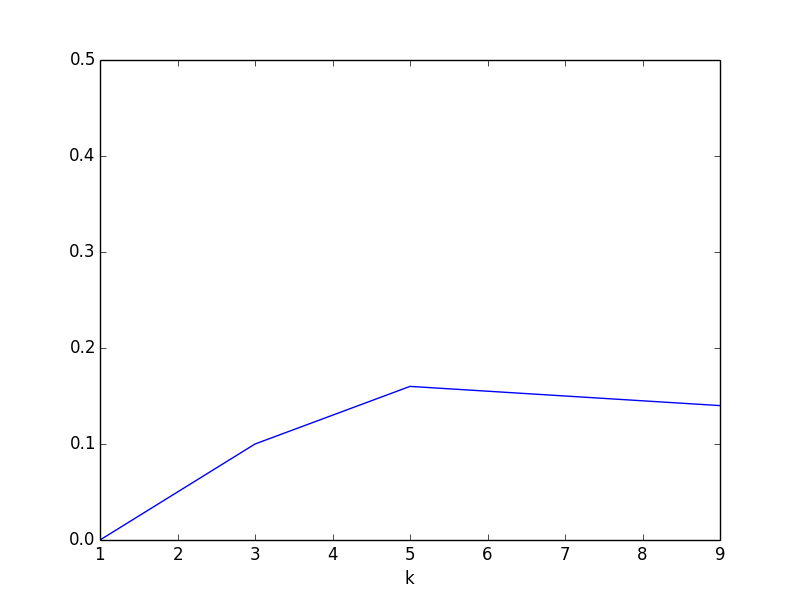
\includegraphics[scale=0.5]{p11.png}
\end{center}
\begin{itemize}
    \item $1$-nearest-neighbor has $E_{in}=0$ because the nearest neighbor of $x_i$ is $x_i$ itself.
    \item $E_{in}$ increases util $k=5$ and decrease a little after.
\end{itemize}

\section*{12}
\begin{center}
    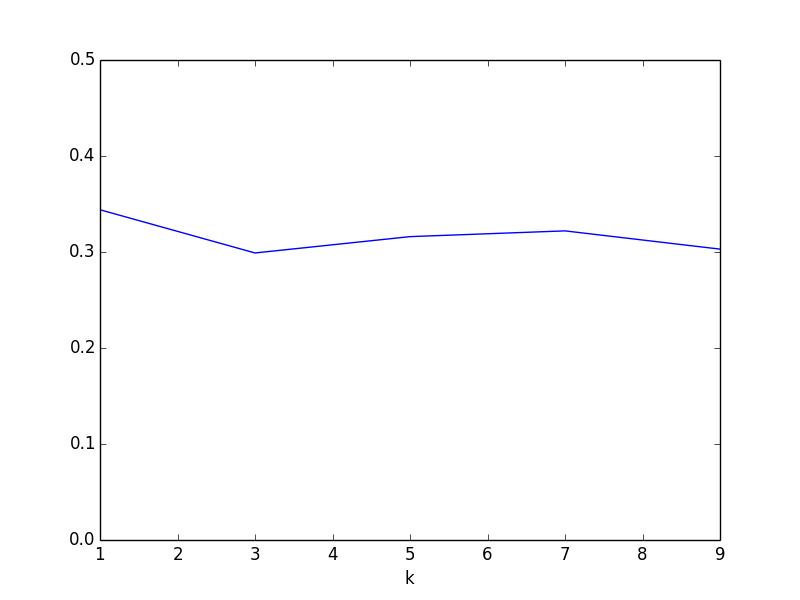
\includegraphics[scale=0.5]{p12.png}
\end{center}
\begin{itemize}
    \item $1$-nearest-neighbor has $E_{in}=0$ but high $E_{out}$ which can be viwe as overfitting.
    \item $E_{out}$ is the lowest when $k=3$.
\end{itemize}

\section*{13}
\begin{center}
    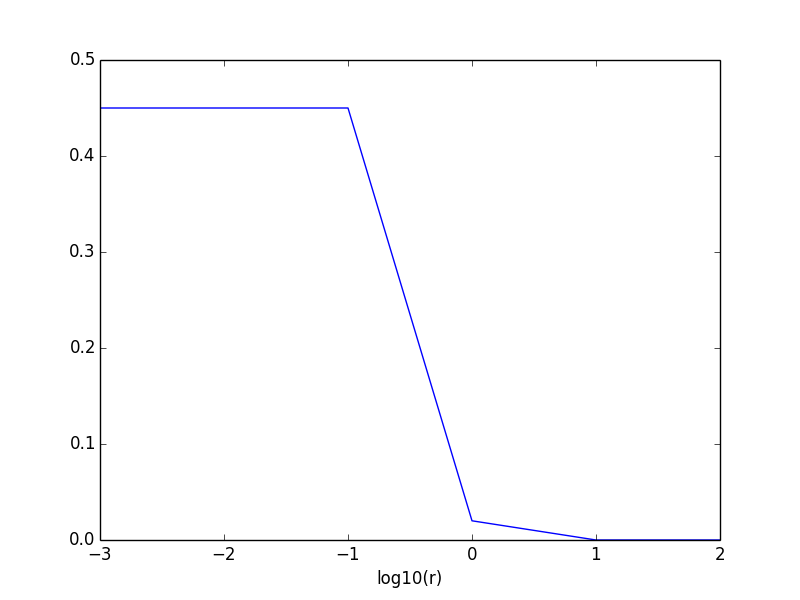
\includegraphics[scale=0.5]{p13.png}
\end{center}
\begin{itemize}
    \item Larger $\gamma$ induce the result of smaller $k$ in k-nearest-neighbors.
    \item $E_{in}=0$ for $\gamma=10, 100$.
    \item Too small $\gamma$ will become average voting by all training data and have bad $E_{in}$.
\end{itemize}
\section*{14}
\begin{center}
    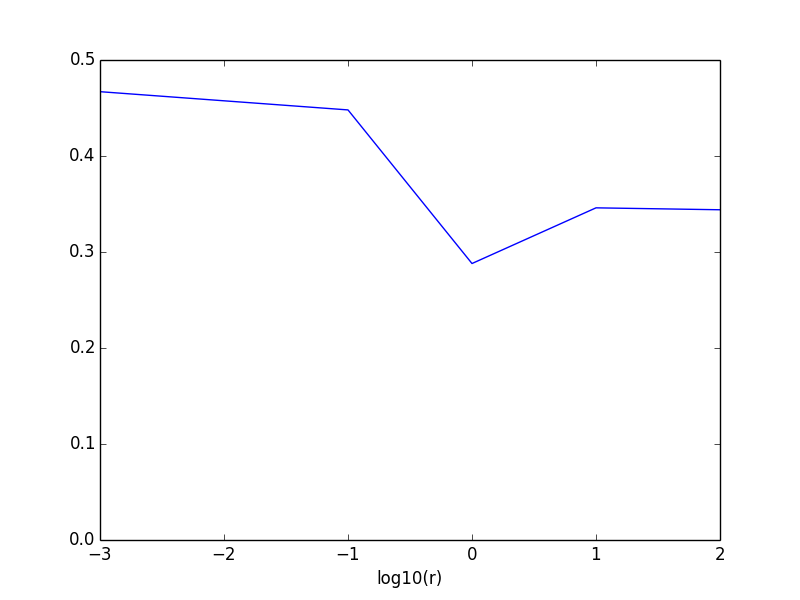
\includegraphics[scale=0.5]{p14.png}
\end{center}
\begin{itemize}
    \item Too large $\gamma$ will overfit on training data.
    \item Too small $\gamma$ will become average voting by all training data and result of bad $E_{out}$.
    \item $E_{out}$ is the lowest when $\gamma=1$.
\end{itemize}

\section*{15}
\begin{center}
    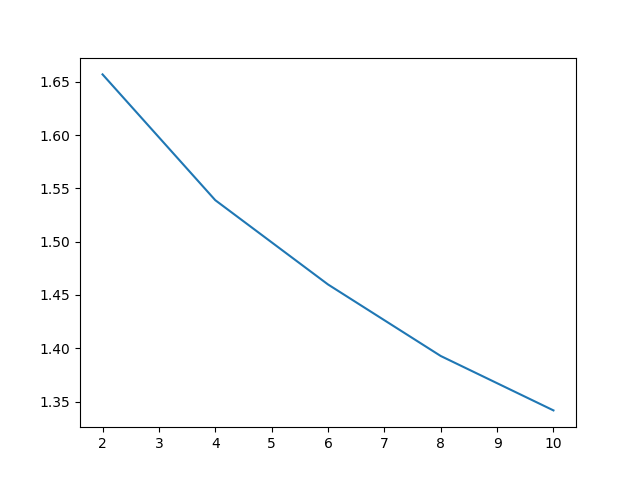
\includegraphics[scale=0.5]{p15.png}
\end{center}
With larger $k$, more centroids means that 
the distance between $x_i$ and its centroid $\mu_m$ will be smaller, 
and the $E_{in}$ will also be smaller.

\section*{16}
\begin{center}
    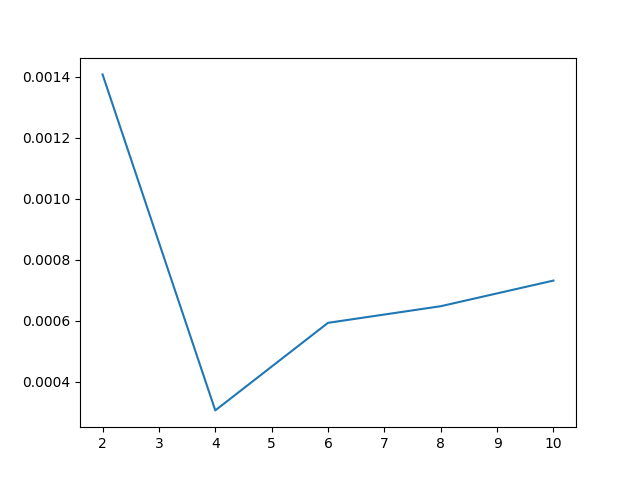
\includegraphics[scale=0.5]{p16.png}
\end{center}
The variances of $E_{in}$ are small even for the randomness of choosing initial $\mu$.
The variance is the smallest when $k=4$.
\section*{17}
\section*{18}
\end{document}


